\begin{figure}
  %\centering
  \begin{subfigure}[t]{0.3\textwidth}
    \caption{Width 5 strong USP.}
  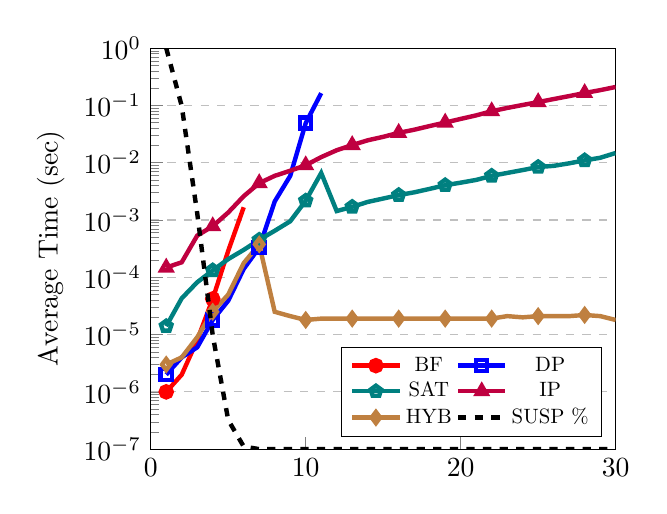
\begin{tikzpicture}
    \begin{axis}[
        scale=.7,
        %title={Average checking time versus puzzle height for 10000 random width 8 puzzles},
        %xlabel={Puzzle Height},
        ylabel={Average Time (sec)},
        %width=3.4in,
        %height=2.5in,
        xmin=0, xmax=30,
        ytick pos=left,
        xtick pos=left,
        ymin=1e-7, ymax=1,
        legend pos=south east,
        legend style={legend columns=2, nodes={scale=0.75, transform shape}},
        ymajorgrids=true,
        grid style=dashed,
        ymode=log,
        cycle list name=color list,
        scale only axis,
        every axis plot/.append style={ultra thick},
      ]
      \addplot[mark=*, mark repeat=3, red]
      coordinates {
(1,0.000001)
(2,0.000002)
(3,0.000008)
(4,0.000042)
(5,0.000290)
(6,0.001668)
      };
      
      
      \addplot[mark=square, mark repeat=3, blue]
      coordinates {
(1,0.000002)
(2,0.000004)
(3,0.000006)
(4,0.000018)
(5,0.000039)
(6,0.000140)
(7,0.000330)
(8,0.002107)
(9,0.005892)
(10,0.049053)
(11,0.163843)
      };
      
      \addplot[mark=pentagon, mark repeat=3, teal]
      coordinates {
(1,0.000014)
(2,0.000043)
(3,0.000082)
(4,0.000132)
(5,0.000208)
(6,0.000301)
(7,0.000451)
(8,0.000649)
(9,0.000950)
(10,0.002174)
(11,0.006619)
(12,0.001433)
(13,0.001696)
(14,0.002068)
(15,0.002371)
(16,0.002722)
(17,0.003043)
(18,0.003496)
(19,0.004051)
(20,0.004487)
(21,0.005012)
(22,0.005906)
(23,0.006633)
(24,0.007448)
(25,0.008406)
(26,0.008819)
(27,0.009764)
(28,0.010991)
(29,0.012199)
(30,0.014788)
      };
      
      \addplot[mark=triangle, mark repeat=3, purple]
      coordinates {
(1,0.000148)
(2,0.000183)
(3,0.000535)
(4,0.000780)
(5,0.001353)
(6,0.002607)
(7,0.004405)
(8,0.005905)
(9,0.007247)
(10,0.009047)
(11,0.012536)
(12,0.016524)
(13,0.020360)
(14,0.024634)
(15,0.028322)
(16,0.033261)
(17,0.037690)
(18,0.043702)
(19,0.050287)
(20,0.058206)
(21,0.067089)
(22,0.079269)
(23,0.090435)
(24,0.101884)
(25,0.114451)
(26,0.129260)
(27,0.145687)
(28,0.164847)
(29,0.184864)
(30,0.210087)
      };

      \addplot[mark=diamond, mark repeat=3, brown]
      coordinates {
(1,0.000003)
(2,0.000004)
(3,0.000009)
(4,0.000025)
(5,0.000050)
(6,0.000177)
(7,0.000376)
(8,0.000025)
(9,0.000021)
(10,0.000018)
(11,0.000019)
(12,0.000019)
(13,0.000019)
(14,0.000019)
(15,0.000019)
(16,0.000019)
(17,0.000019)
(18,0.000019)
(19,0.000019)
(20,0.000019)
(21,0.000019)
(22,0.000019)
(23,0.000021)
(24,0.000020)
(25,0.000021)
(26,0.000021)
(27,0.000021)
(28,0.000022)
(29,0.000021)
(30,0.000018)
      };
      \addplot[style=dashed, black]
      coordinates{
        (0,0)
        (0,1)
      };
      \legend{BF, DP, SAT, IP, HYB, SUSP \%}
    \end{axis}
    \begin{axis}[
        scale only axis,
        scale=.7,
        %width=3.4in,
        %height=2.5in,
        %axis y line*=right,
        axis y line=none,
        ymin=0,ymax=100,
        xmin=0,xmax=30,
        axis x line=none,
        every axis plot/.append style={ultra thick},
        %ylabel={Percent SUSP},
        axis x line=none,
        ylabel style = {align=center},ylabel near ticks
        ]
      \addplot[style=dashed]
      coordinates {
(1,100.0)
(2,85.56)
(3,58.8)
(4,28.410000000000004)
(5,7.2700000000000005)
(6,0.65)
(7,0.0)
(8,0.0)
(9,0.0)
(10,0.0)
(11,0.0)
(12,0.0)
(13,0.0)
(14,0.0)
(15,0.0)
(16,0.0)
(17,0.0)
(18,0.0)
(19,0.0)
(20,0.0)
(21,0.0)
(22,0.0)
(23,0.0)
(24,0.0)
(25,0.0)
(26,0.0)
(27,0.0)
(28,0.0)
(29,0.0)
(30,0.0)
      }; %\label{percentSUSP}
      %\legend{SUSP \%}
    \end{axis}
  \end{tikzpicture}

  \end{subfigure}%
  ~~~~~~~~~~~~~~~~~~~~~~~~~~~~~~~~~~
  \begin{subfigure}[t]{0.3\textwidth}
      \caption{Width 6 strong USP.}
  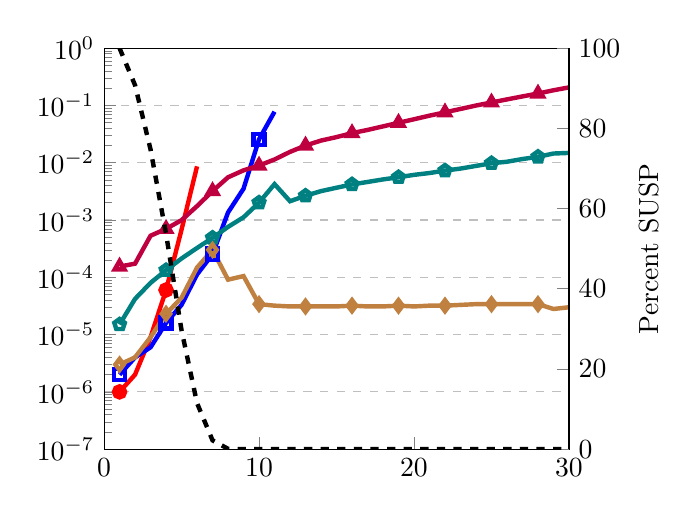
\begin{tikzpicture}
    \begin{axis}[
        scale=.7,
        %title={Average checking time versus puzzle height for 10000 random width 8 puzzles},
        %xlabel={Puzzle Height},
        %ylabel={Average Time (sec)},
        %width=3.4in,
        %height=2.5in,
        xmin=0, xmax=30,
        ytick pos=left,
        xtick pos=left,
        ymin=1e-7, ymax=1,
        legend pos=south east,
        legend style={legend columns=2},
        ymajorgrids=true,
        grid style=dashed,
        ymode=log,
        cycle list name=color list,
        scale only axis,
        every axis plot/.append style={ultra thick},
      ]
      
      \addplot[mark=*, mark repeat=3, red]
      coordinates {
(1,0.000001)
(2,0.000002)
(3,0.000009)
(4,0.000060)
(5,0.000679)
(6,0.008650)
      };
      
      
      \addplot[mark=square, mark repeat=3, blue]
      coordinates {
(1,0.000002)
(2,0.000004)
(3,0.000006)
(4,0.000016)
(5,0.000033)
(6,0.000112)
(7,0.000253)
(8,0.001355)
(9,0.003520)
(10,0.025636)
(11,0.077827)
      };
      
      \addplot[mark=pentagon, mark repeat=3, teal]
      coordinates {
(1,0.000015)
(2,0.000042)
(3,0.000080)
(4,0.000133)
(5,0.000213)
(6,0.000325)
(7,0.000489)
(8,0.000758)
(9,0.001117)
(10,0.002009)
(11,0.004235)
(12,0.002129)
(13,0.002650)
(14,0.003195)
(15,0.003661)
(16,0.004184)
(17,0.004614)
(18,0.005113)
(19,0.005574)
(20,0.006143)
(21,0.006614)
(22,0.007291)
(23,0.007908)
(24,0.008801)
(25,0.009797)
(26,0.010409)
(27,0.011608)
(28,0.012684)
(29,0.014477)
(30,0.014838)
      };
      
      \addplot[mark=triangle, mark repeat=3, purple]
      coordinates {
(1,0.000154)
(2,0.000173)
(3,0.000532)
(4,0.000701)
(5,0.000994)
(6,0.001749)
(7,0.003201)
(8,0.005568)
(9,0.007367)
(10,0.008928)
(11,0.011399)
(12,0.015474)
(13,0.019977)
(14,0.024378)
(15,0.028027)
(16,0.032904)
(17,0.037362)
(18,0.043104)
(19,0.049805)
(20,0.057387)
(21,0.066355)
(22,0.075801)
(23,0.086858)
(24,0.099631)
(25,0.112705)
(26,0.127511)
(27,0.143807)
(28,0.161481)
(29,0.184042)
(30,0.206666)
      };

      \addplot[mark=diamond, mark repeat=3, brown]
      coordinates {
(1,0.000003)
(2,0.000004)
(3,0.000009)
(4,0.000023)
(5,0.000044)
(6,0.000148)
(7,0.000301)
(8,0.000091)
(9,0.000105)
(10,0.000034)
(11,0.000032)
(12,0.000031)
(13,0.000031)
(14,0.000031)
(15,0.000031)
(16,0.000032)
(17,0.000031)
(18,0.000031)
(19,0.000032)
(20,0.000031)
(21,0.000032)
(22,0.000032)
(23,0.000033)
(24,0.000034)
(25,0.000034)
(26,0.000034)
(27,0.000034)
(28,0.000034)
(29,0.000028)
(30,0.000030)
      };
      %\legend{BF, DP, SAT, IP, Hybrid}
    \end{axis}
    \begin{axis}[
        scale only axis,
        scale=.7,
        %width=3.4in,
        %height=2.5in,
        axis y line*=right,
        ymin=0,ymax=100,
        xmin=0,xmax=30,
        axis x line=none,
        every axis plot/.append style={ultra thick},
        ylabel={Percent SUSP},
        axis x line=none,
        ylabel style = {align=center},ylabel near ticks
        ]
      \addplot[style=dashed]
      coordinates {
        (1,100.0)
(2,90.75999999999999)
(3,74.72999999999999)
(4,53.690000000000005)
(5,29.65)
(6,11.48)
(7,2.19)
(8,0.08)
(9,0.01)
(10,0.0)
(11,0.0)
(12,0.0)
(13,0.0)
(14,0.0)
(15,0.0)
(16,0.0)
(17,0.0)
(18,0.0)
(19,0.0)
(20,0.0)
(21,0.0)
(22,0.0)
(23,0.0)
(24,0.0)
(25,0.0)
(26,0.0)
(27,0.0)
(28,0.0)
(29,0.0)
(30,0.0)
      }; %\label{percentSUSP}
      %\legend{SUSP \%}
    \end{axis}
  \end{tikzpicture}

  \end{subfigure}

  \begin{subfigure}[t]{0.3\textwidth}
    \vspace{1.5ex}
    \caption{Width 7 strong USP.}
  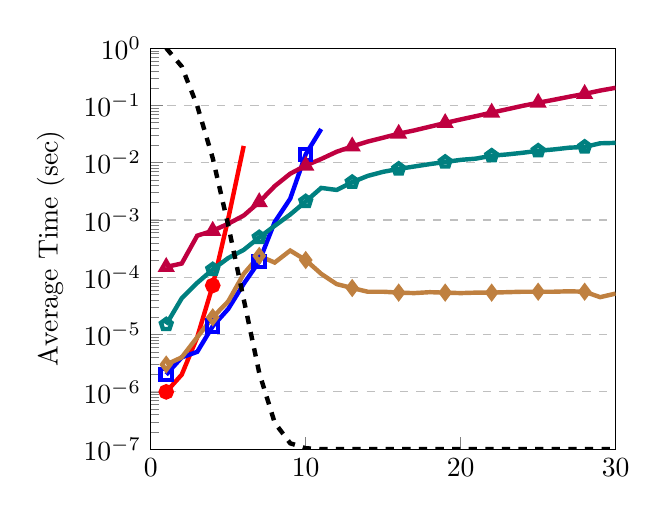
\begin{tikzpicture}
    \begin{axis}[
        scale=.7,
        %title={Average checking time versus puzzle height for 10000 random width 8 puzzles},
        %xlabel={Puzzle Height},
        ylabel={Average Time (sec)},
        %width=3.4in,
        %height=2.5in,
        xmin=0, xmax=30,
        ytick pos=left,
        xtick pos=left,
        ymin=1e-7, ymax=1,
        legend pos=south east,
        legend style={legend columns=2},
        ymajorgrids=true,
        grid style=dashed,
        ymode=log,
        cycle list name=color list,
        scale only axis,
        every axis plot/.append style={ultra thick},
      ]
      
      \addplot[mark=*, mark repeat=3, red]
      coordinates {
(1,0.000001)
(2,0.000002)
(3,0.000009)
(4,0.000072)
(5,0.001053)
(6,0.019641)
      };
      
      
      \addplot[mark=square, mark repeat=3, blue]
      coordinates {
        (1,0.000002)
(2,0.000004)
(3,0.000005)
(4,0.000014)
(5,0.000028)
(6,0.000077)
(7,0.000189)
(8,0.000923)
(9,0.002358)
(10,0.014033)
(11,0.038762)
      };
      
      \addplot[mark=pentagon, mark repeat=3, teal]
      coordinates {
(1,0.000015)
(2,0.000043)
(3,0.000080)
(4,0.000137)
(5,0.000217)
(6,0.000301)
(7,0.000497)
(8,0.000792)
(9,0.001247)
(10,0.002107)
(11,0.003634)
(12,0.003348)
(13,0.004578)
(14,0.005887)
(15,0.006944)
(16,0.007799)
(17,0.008594)
(18,0.009459)
(19,0.010304)
(20,0.011223)
(21,0.011809)
(22,0.013254)
(23,0.013968)
(24,0.014924)
(25,0.016176)
(26,0.017060)
(27,0.018297)
(28,0.018889)
(29,0.021833)
(30,0.022220)
      };
      
      \addplot[mark=triangle, mark repeat=3, purple]
      coordinates {
(1,0.000152)
(2,0.000174)
(3,0.000533)
(4,0.000649)
(5,0.000861)
(6,0.001198)
(7,0.002055)
(8,0.003904)
(9,0.006433)
(10,0.008940)
(11,0.011625)
(12,0.015559)
(13,0.019298)
(14,0.023393)
(15,0.027376)
(16,0.032076)
(17,0.036646)
(18,0.042521)
(19,0.049422)
(20,0.056971)
(21,0.065176)
(22,0.074952)
(23,0.085829)
(24,0.098522)
(25,0.111465)
(26,0.125384)
(27,0.141956)
(28,0.159088)
(29,0.181931)
(30,0.203126)
      };

      \addplot[mark=diamond, mark repeat=3, brown]
      coordinates {
(1,0.000003)
(2,0.000004)
(3,0.000009)
(4,0.000020)
(5,0.000038)
(6,0.000115)
(7,0.000236)
(8,0.000181)
(9,0.000293)
(10,0.000200)
(11,0.000115)
(12,0.000076)
(13,0.000065)
(14,0.000056)
(15,0.000056)
(16,0.000054)
(17,0.000053)
(18,0.000055)
(19,0.000054)
(20,0.000053)
(21,0.000054)
(22,0.000054)
(23,0.000055)
(24,0.000056)
(25,0.000056)
(26,0.000056)
(27,0.000057)
(28,0.000056)
(29,0.000045)
(30,0.000052)
      };
      \addplot[style=dashed, black]
      coordinates{
        (0,0)
        (0,1)
      };
      %\legend{BF, DP, SAT, IP, Hybrid, SUSP \%}
    \end{axis}
    \begin{axis}[
        scale only axis,
        scale=.7,
        %width=3.4in,
        %height=2.5in,
        %axis y line*=right,
        axis y line=none,
        ymin=0,ymax=100,
        xmin=0,xmax=30,
        axis x line=none,
        every axis plot/.append style={ultra thick},
        %ylabel={Percent SUSP},
        axis x line=none,
        ylabel style = {align=center},ylabel near ticks
        ]
      \addplot[style=dashed]
      coordinates {
(1,100.0)
(2,95.44)
(3,85.61999999999999)
(4,72.59)
(5,55.82)
(6,37.38)
(7,19.040000000000003)
(8,6.59)
(9,1.47)
(10,0.22)
(11,0.01)
(12,0.0)
(13,0.0)
(14,0.0)
(15,0.0)
(16,0.0)
(17,0.0)
(18,0.0)
(19,0.0)
(20,0.0)
(21,0.0)
(22,0.0)
(23,0.0)
(24,0.0)
(25,0.0)
(26,0.0)
(27,0.0)
(28,0.0)
(29,0.0)
(30,0.0)
      }; %\label{percentSUSP}
      %\legend{SUSP \%}
    \end{axis}
  \end{tikzpicture}

  \end{subfigure}%
  ~~~~~~~~~~~~~~~~~~~~~~~~~~~~~~~~~~
  \begin{subfigure}[t]{0.3\textwidth}
    \vspace{1.5ex}
    \caption{Width 8 strong USP.}
  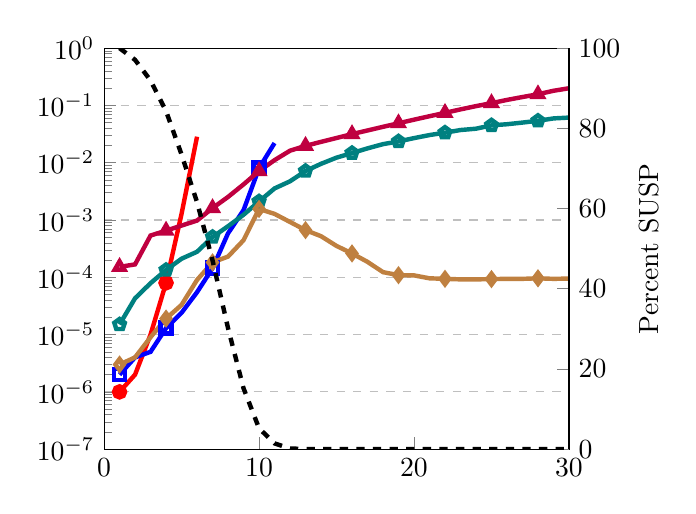
\begin{tikzpicture}
    \begin{axis}[
        scale=.7,
        %title={Average checking time versus puzzle height for 10000 random width 8 puzzles},
        %xlabel={Puzzle Height},
        %ylabel={Average Time (sec)},
        %width=3.4in,
        %height=2.5in,
        xmin=0, xmax=30,
        ytick pos=left,
        xtick pos=left,
        ymin=1e-7, ymax=1,
        legend pos=south east,
        legend style={legend columns=2},
        ymajorgrids=true,
        grid style=dashed,
        ymode=log,
        cycle list name=color list,
        scale only axis,
        every axis plot/.append style={ultra thick},
      ]
      
      \addplot[mark=*, mark repeat=3, red]
      coordinates {
(1,0.000001)
(2,0.000002)
(3,0.000010)
(4,0.000080)
(5,0.001278)
(6,0.028475)
      };
      
      
      \addplot[mark=square, mark repeat=3, blue]
      coordinates {
(1,0.000002)
(2,0.000004)
(3,0.000005)
(4,0.000013)
(5,0.000024)
(6,0.000055)
(7,0.000144)
(8,0.000586)
(9,0.001485)
(10,0.008024)
(11,0.022047)
      };
      
      \addplot[mark=pentagon, mark repeat=3, teal]
      coordinates {
(1,0.000015)
(2,0.000043)
(3,0.000079)
(4,0.000134)
(5,0.000211)
(6,0.000279)
(7,0.000505)
(8,0.000779)
(9,0.001235)
(10,0.002107)
(11,0.003558)
(12,0.004742)
(13,0.007168)
(14,0.009571)
(15,0.012269)
(16,0.014747)
(17,0.017819)
(18,0.021106)
(19,0.023533)
(20,0.026900)
(21,0.030405)
(22,0.033466)
(23,0.037229)
(24,0.039283)
(25,0.044903)
(26,0.046999)
(27,0.050242)
(28,0.053942)
(29,0.059373)
(30,0.061401)
      };
      
      \addplot[mark=triangle, mark repeat=3, purple]
      coordinates {
(1,0.000152)
(2,0.000168)
(3,0.000536)
(4,0.000653)
(5,0.000800)
(6,0.000978)
(7,0.001614)
(8,0.002529)
(9,0.004187)
(10,0.007130)
(11,0.011094)
(12,0.016223)
(13,0.019727)
(14,0.023134)
(15,0.026999)
(16,0.031622)
(17,0.036585)
(18,0.042355)
(19,0.048855)
(20,0.056438)
(21,0.064877)
(22,0.074264)
(23,0.085323)
(24,0.097307)
(25,0.109676)
(26,0.124883)
(27,0.140305)
(28,0.156828)
(29,0.180271)
(30,0.199624)
      };

      \addplot[mark=diamond, mark repeat=3, brown]
      coordinates {
(1,0.000003)
(2,0.000004)
(3,0.000009)
(4,0.000019)
(5,0.000033)
(6,0.000090)
(7,0.000182)
(8,0.000230)
(9,0.000444)
(10,0.001559)
(11,0.001280)
(12,0.000924)
(13,0.000666)
(14,0.000522)
(15,0.000353)
(16,0.000261)
(17,0.000186)
(18,0.000123)
(19,0.000109)
(20,0.000108)
(21,0.000096)
(22,0.000094)
(23,0.000092)
(24,0.000092)
(25,0.000093)
(26,0.000094)
(27,0.000094)
(28,0.000096)
(29,0.000094)
(30,0.000095)
      };
      %\legend{BF, DP, SAT, IP, Hybrid}
    \end{axis}
    \begin{axis}[
        scale only axis,
        scale=.7,
        %width=3.4in,
        %height=2.5in,
        axis y line*=right,
        ymin=0,ymax=100,
        xmin=0,xmax=30,
        axis x line=none,
        every axis plot/.append style={ultra thick},
        ylabel={Percent SUSP},
        axis x line=none,
        ylabel style = {align=center},ylabel near ticks
        ]
      \addplot[style=dashed]
      coordinates {
(1,100.0)
(2,97.08)
(3,91.94)
(4,84.31)
(5,73.49)
(6,61.59)
(7,47.099999999999994)
(8,30.18)
(9,15.18)
(10,5.21)
(11,1.44)
(12,0.16999999999999998)
(13,0.02)
(14,0.0)
(15,0.0)
(16,0.0)
(17,0.0)
(18,0.0)
(19,0.0)
(20,0.0)
(21,0.0)
(22,0.0)
(23,0.0)
(24,0.0)
(25,0.0)
(26,0.0)
(27,0.0)
(28,0.0)
(29,0.0)
(30,0.0)
      }; %\label{percentSUSP}
      %\legend{SUSP \%}
    \end{axis}
  \end{tikzpicture}
  \end{subfigure}



  \begin{subfigure}[t]{0.3\textwidth}
    \vspace{1.5ex}
    \caption{Width 9 strong USP.}
  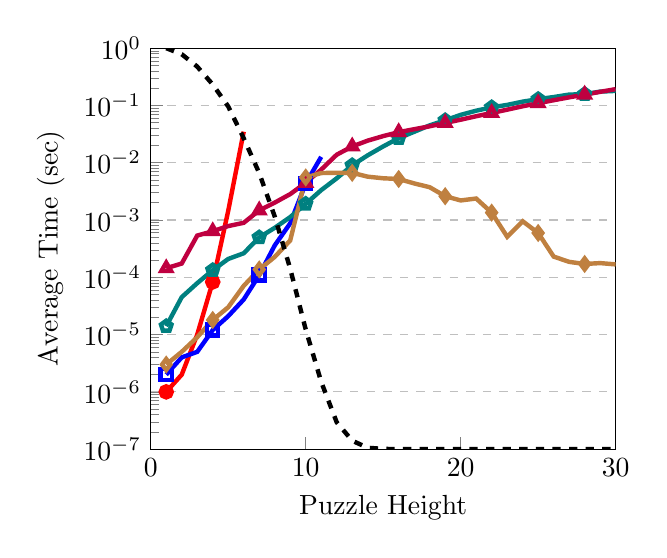
\begin{tikzpicture}
    \begin{axis}[
        scale=.7,
        %title={Average checking time versus puzzle height for 10000 random width 8 puzzles},
        xlabel={Puzzle Height},
        ylabel={Average Time (sec)},
        %width=3.4in,
        %height=2.5in,
        xmin=0, xmax=30,
        ytick pos=left,
        xtick pos=left,
        ymin=1e-7, ymax=1,
        legend pos=south east,
        legend style={legend columns=2},
        ymajorgrids=true,
        grid style=dashed,
        ymode=log,
        cycle list name=color list,
        scale only axis,
        every axis plot/.append style={ultra thick},
      ]
      
      \addplot[mark=*, mark repeat=3, red]
      coordinates {
(1,0.000001)
(2,0.000002)
(3,0.000010)
(4,0.000083)
(5,0.001447)
(6,0.034856)
      };
      
      
      \addplot[mark=square, mark repeat=3, blue]
      coordinates {
(1,0.000002)
(2,0.000004)
(3,0.000005)
(4,0.000012)
(5,0.000021)
(6,0.000041)
(7,0.000109)
(8,0.000360)
(9,0.000876)
(10,0.004350)
(11,0.012662)
      };
      
      \addplot[mark=pentagon, mark repeat=3, teal]
      coordinates {
(1,0.000014)
(2,0.000045)
(3,0.000079)
(4,0.000133)
(5,0.000209)
(6,0.000263)
(7,0.000497)
(8,0.000731)
(9,0.001125)
(10,0.001914)
(11,0.003326)
(12,0.005342)
(13,0.009016)
(14,0.013461)
(15,0.019261)
(16,0.026867)
(17,0.034681)
(18,0.044907)
(19,0.055021)
(20,0.068536)
(21,0.080987)
(22,0.092563)
(23,0.102250)
(24,0.116448)
(25,0.128873)
(26,0.140122)
(27,0.154784)
(28,0.157334)
(29,0.174383)
(30,0.179453)
      };
      
      \addplot[mark=triangle, mark repeat=3, purple]
      coordinates {
(1,0.000144)
(2,0.000174)
(3,0.000535)
(4,0.000637)
(5,0.000784)
(6,0.000894)
(7,0.001474)
(8,0.002012)
(9,0.002833)
(10,0.004460)
(11,0.007585)
(12,0.013803)
(13,0.019238)
(14,0.024299)
(15,0.029166)
(16,0.034196)
(17,0.038492)
(18,0.043241)
(19,0.049450)
(20,0.056393)
(21,0.064838)
(22,0.073858)
(23,0.084390)
(24,0.096774)
(25,0.109239)
(26,0.123410)
(27,0.138516)
(28,0.154470)
(29,0.172965)
(30,0.192481)
      };

      \addplot[mark=diamond, mark repeat=3, brown]
      coordinates {
(1,0.000003)
(2,0.000005)
(3,0.000009)
(4,0.000018)
(5,0.000030)
(6,0.000071)
(7,0.000137)
(8,0.000227)
(9,0.000440)
(10,0.005532)
(11,0.006604)
(12,0.006680)
(13,0.006660)
(14,0.005714)
(15,0.005352)
(16,0.005199)
(17,0.004353)
(18,0.003739)
(19,0.002604)
(20,0.002197)
(21,0.002372)
(22,0.001346)
(23,0.000511)
(24,0.000952)
(25,0.000594)
(26,0.000230)
(27,0.000186)
(28,0.000171)
(29,0.000177)
(30,0.000168)
      };
      \addplot[style=dashed, black]
      coordinates{
        (0,0)
        (0,1)
      };
      %\legend{BF, DP, SAT, IP, Hybrid, SUSP \%}
    \end{axis}
    \begin{axis}[
        scale only axis,
        scale=.7,
        %width=3.4in,
        %height=2.5in,
        %axis y line*=right,
        axis y line=none,
        ymin=0,ymax=100,
        xmin=0,xmax=30,
        axis x line=none,
        every axis plot/.append style={ultra thick},
        %ylabel={Percent SUSP},
        axis x line=none,
        ylabel style = {align=center},ylabel near ticks
        ]
      \addplot[style=dashed]
      coordinates {
(1,100.0)
(2,98.48)
(3,95.39999999999999)
(4,90.94)
(5,85.47)
(6,77.53)
(7,68.85)
(8,58.040000000000006)
(9,45.01)
(10,29.86)
(11,16.78)
(12,6.710000000000001)
(13,2.11)
(14,0.33999999999999997)
(15,0.06999999999999999)
(16,0.0)
(17,0.0)
(18,0.0)
(19,0.0)
(20,0.0)
(21,0.0)
(22,0.0)
(23,0.0)
(24,0.0)
(25,0.0)
(26,0.0)
(27,0.0)
(28,0.0)
(29,0.0)
(30,0.0)
      }; %\label{percentSUSP}
      %\legend{SUSP \%}
    \end{axis}
  \end{tikzpicture}

  \end{subfigure}%
  ~~~~~~~~~~~~~~~~~~~~~~~~~~~~~~~~~~
  \begin{subfigure}[t]{0.3\textwidth}
    \vspace{1.5ex}
    \caption{Width 10 strong USP.}
  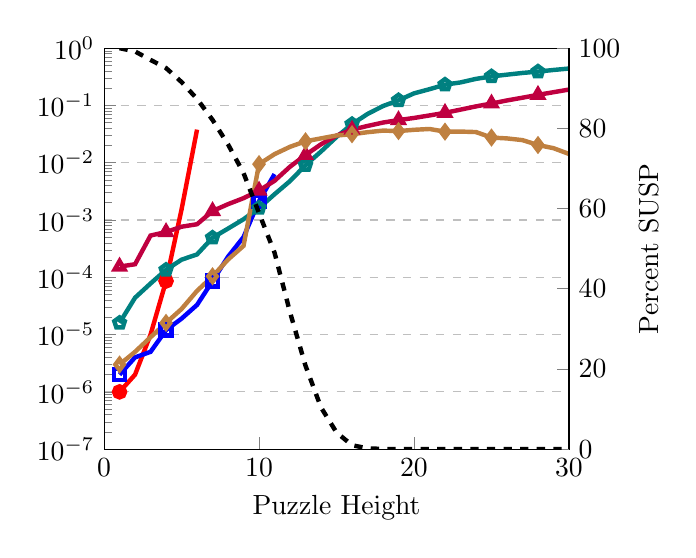
\begin{tikzpicture}
    \begin{axis}[
        scale=.7,
        %title={Average checking time versus puzzle height for 10000 random width 8 puzzles},
        xlabel={Puzzle Height},
        %ylabel={Average Time (sec)},
        %width=3.4in,
        %height=2.5in,
        xmin=0, xmax=30,
        ytick pos=left,
        xtick pos=left,
        ymin=1e-7, ymax=1,
        legend pos=south east,
        legend style={legend columns=2},
        ymajorgrids=true,
        grid style=dashed,
        ymode=log,
        cycle list name=color list,
        scale only axis,
        every axis plot/.append style={ultra thick},
      ]
      
      \addplot[mark=*, mark repeat=3, red]
      coordinates {
(1,0.000001)
(2,0.000002)
(3,0.000010)
(4,0.000086)
(5,0.001527)
(6,0.037871)
      };
      
      
      \addplot[mark=square, mark repeat=3, blue]
      coordinates {
(1,0.000002)
(2,0.000004)
(3,0.000005)
(4,0.000012)
(5,0.000019)
(6,0.000033)
(7,0.000086)
(8,0.000229)
(9,0.000504)
(10,0.002137)
(11,0.006329)
      };
      
      \addplot[mark=pentagon, mark repeat=3, teal]
      coordinates {
(1,0.000016)
(2,0.000044)
(3,0.000078)
(4,0.000135)
(5,0.000203)
(6,0.000251)
(7,0.000491)
(8,0.000709)
(9,0.001031)
(10,0.001623)
(11,0.002816)
(12,0.004783)
(13,0.009073)
(14,0.015697)
(15,0.028175)
(16,0.047146)
(17,0.070970)
(18,0.097643)
(19,0.122891)
(20,0.162530)
(21,0.192221)
(22,0.230472)
(23,0.252367)
(24,0.291011)
(25,0.321245)
(26,0.344867)
(27,0.369262)
(28,0.389873)
(29,0.416138)
(30,0.441104)
      };
      
      \addplot[mark=triangle, mark repeat=3, purple]
      coordinates {
(1,0.000154)
(2,0.000169)
(3,0.000536)
(4,0.000617)
(5,0.000764)
(6,0.000844)
(7,0.001435)
(8,0.001891)
(9,0.002407)
(10,0.003265)
(11,0.004831)
(12,0.008536)
(13,0.013664)
(14,0.021003)
(15,0.029735)
(16,0.037749)
(17,0.043829)
(18,0.050243)
(19,0.055525)
(20,0.060482)
(21,0.066943)
(22,0.074377)
(23,0.084496)
(24,0.096253)
(25,0.108099)
(26,0.122322)
(27,0.136572)
(28,0.153064)
(29,0.170231)
(30,0.189359)
      };

      \addplot[mark=diamond, mark repeat=3, brown]
      coordinates {
(1,0.000003)
(2,0.000005)
(3,0.000009)
(4,0.000016)
(5,0.000028)
(6,0.000058)
(7,0.000104)
(8,0.000204)
(9,0.000354)
(10,0.009436)
(11,0.014118)
(12,0.018966)
(13,0.023669)
(14,0.026621)
(15,0.029888)
(16,0.031436)
(17,0.034132)
(18,0.036392)
(19,0.035710)
(20,0.037570)
(21,0.038830)
(22,0.034886)
(23,0.035004)
(24,0.034309)
(25,0.027510)
(26,0.026576)
(27,0.024817)
(28,0.020389)
(29,0.017953)
(30,0.014241)
      };
      %\legend{BF, DP, SAT, IP, Hybrid}
    \end{axis}
    \begin{axis}[
        scale only axis,
        scale=.7,
        %width=3.4in,
        %height=2.5in,
        axis y line*=right,
        ymin=0,ymax=100,
        xmin=0,xmax=30,
        axis x line=none,
        every axis plot/.append style={ultra thick},
        ylabel={Percent SUSP},
        axis x line=none,
        ylabel style = {align=center},ylabel near ticks
        ]
      \addplot[style=dashed]
      coordinates {
(1,100.0)
(2,99.18)
(3,97.07000000000001)
(4,95.04)
(5,91.55)
(6,87.35000000000001)
(7,82.11)
(8,76.0)
(9,68.86)
(10,58.87)
(11,49.02)
(12,34.14)
(13,20.8)
(14,10.4)
(15,4.17)
(16,0.98)
(17,0.21)
(18,0.04)
(19,0.0)
(20,0.0)
(21,0.0)
(22,0.0)
(23,0.0)
(24,0.0)
(25,0.0)
(26,0.0)
(27,0.0)
(28,0.0)
(29,0.0)
(30,0.0)
      }; %\label{percentSUSP}
      %\legend{SUSP \%}
    \end{axis}
  \end{tikzpicture}
  \end{subfigure}

  \vspace{-2ex}
  \caption{Log plots of the average running times for verifying 10000 random puzzles of widths
    five to ten. Note that the legend in (a) applies to all six plots,
    and that the axes are named only the edge of the page.  Each plot
    describes the behavior of five algorithms brute force (BF),
    dynamic programming (DP), reduction to satisfiability (SAT),
    reduction to integer programming (IP), and the hybrid algorithm
    (HYB).  The final dashed line indicates the percentage of SUSP
    found among the 10000 random puzzles.}
  \label{fig:perform}
\end{figure}
  
